\documentclass[10pt]{article} 

\usepackage[utf8]{inputenc}
\usepackage[T1]{fontenc}
\usepackage{lmodern}
\usepackage{graphicx}
\usepackage{color}
\usepackage{hyperref}
\usepackage{amsmath}
\usepackage{amsfonts}
\usepackage{epstopdf}
\usepackage[table]{xcolor}
\usepackage{amsmath,amsthm,amssymb, tikz}
\usepackage{mathtools}
\usepackage{titlesec}
\usepackage{float}
\usepackage[margin=1in]{geometry}

\sloppy
\epstopdfsetup{outdir=./}

%
\setlength{\paperwidth}{21cm}   % A4
\setlength{\paperheight}{29.7cm}% A4
\setlength\topmargin{-0.5cm}    
\setlength\oddsidemargin{0cm}   
\setlength\textheight{24.7cm} 
\setlength\textwidth{16.0cm}
\setlength\columnsep{0.6cm}  
\newlength\titlebox 
\setlength\titlebox{5cm}
\setlength\headheight{5pt}   
\setlength\headsep{0pt}




\flushbottom \twocolumn \sloppy


\titleformat{\section}[block]
{\fontsize{13}{16}\bfseries}
{\thesection}
{1em}
{\MakeUppercase}
\titleformat{\subsection}[hang]
{\fontsize{12}{15}\bfseries}
{\thesubsection}
{1em}
{}

\graphicspath{{../outputs/}}


\renewenvironment{abstract}%
{\centerline{\large\bf Abstract}%
    \begin{list}{}%
        {\setlength{\rightmargin}{0.6cm}%
            \setlength{\leftmargin}{0.6cm}}%
        \item[]\ignorespaces%
        \small
    }%
    {\unskip\end{list}}


\begin{document}
    \title{Image Encryption Techniques with Chaotic Systems\\
        \large McGill University, Math 326} 
    
    \author{William Tang, 260924573} 
    
    \date{\today}
    
    \maketitle
    
    
    
    \begin{abstract}
        In this project, we investigate how the chaotic logistic map can be applied to image encryption. A basic method of image encryption is introduced along with variants using discrete chaotic maps. We then propose a new image encryption scheme based on a forward/backward logistic map iteration of the pixels of a given image. Overall conclusions were drawn by qualititatively analyzing the sensitivity of each method, comparing image histograms, and comparing run time performance. Basic methods of image encryption were found to be relatively effective and offer an alternative to fast, real-time encryption. However, we found that our new method may not be optimal in terms of the computing power required and in key sensitivity, thus wiping out some of the motivations of using a discrete chaotic map in the first place. 
    \end{abstract}
    
    \section{Introduction}
    
    As society moves increasingly closer to an all-encompassing digital world, secure and reliable cryptosystems have been at the heart of many concerns. It is important that information be transferred safely when needed. In this project, we explored this topic in the context of image encryption and how the chaotic logistic map can be applied to it. We then investigated a new image encryption scheme based on a forward/backward logistic map iteration of the pixels of a given image. Overall conclusions
    were drawn by qualititatively analyzing the sensitivity of each method, comparing image histograms, and comparing run time performance. We find that our new method may not be optimal in terms of the computing power required and in key sensitivity, thus wiping out some of the motivations of using a discrete chaotic map in the first place. Nevertheless, the use of chaotic maps in encryption remains enticing.
    
    \section{Related Work}
    
    Many advanced methods of encryption involving the use of chaotic systems have been studied for quite a while and as such, this paper only serves as an extreme simplification or basic introduction to actual encryption techniques. \\
    
    As early as 2006, Pareek et al. proposed their image encryption scheme using two chaotic logistic maps alongside an external 80-bit secret key \cite{PAREEK2006926}. In fact, the authors suggested that using such methods may be more useful for real-time image encryption over traditional methods. Therefore, because many chaotic maps are simple functions and may be iterated quickly with modern hardware, a common interest in using chaos in encryption is that it provides a fast process that would be suitable for real-time applications (and perhaps better than traditional methods of encryption like AES). In order to ensure the security of such approaches in this domain, studies have combined the logistic map with additional procedures, such as encrypting an image using the Hartley transform and logistic map \cite{Singh}.\\
    
    Other approaches have explored dynamical systems outside of a simple logistic map. For example, there have been successful attempts at using the Hénon Map and Arnold Cat Map to encrypt images, where the authors guarantee that ``the cryptosystem can work effectively in real-time applications'' \cite{Ahmad}. Modern encryption schemes that make use of discrete chaotic maps today are quite secure, being able to resist statistical attacks, plaintext attacks, and brute force attacks.  
    
    \section{Methods}
    
    As one can see, there is genuine interest in using discrete chaotic maps as an alternative to more popular encryption schemes. In this section, we introduce simplified encryption schemes using chaotic systems. These would not be safe in any real-world setting, but instead serve as an educational tool.
    
    \subsection{One-time Pad}
    
    
    The concept of the one-time pad encryption method is used in cryptography to create ciphertext that is theoretically impossible to break \cite{Bellovin}. This method involves generating a key and using it to encode the message. The same key is used to decode the message. There are 4 different conditions that are required by this technique:
    \begin{itemize}
        \item The key must be truly random.
        \item The key has to be at least as long as the message to encrypt.
        \item We cannot reuse the key.
        \item We cannot share the key (except for the intended receivers/senders of the message).
    \end{itemize}

     In reality, it may be difficult, or even impossible to implement some of the requirements of the one-time pad. It may be hard to guarantee that the key will not be shared or leaked to any other parties. However, this does not mean the one-time pad is completely useless. For example, its concepts may be utilized in quantum cryptography, in a component aptly named \textit{one-time quantum pad} \cite{Brassard2005}.\\
     
     This project's methods are also based on the idea of a one-time pad encryption, using a stream cipher.

   
    
    \subsection{XOR Cipher} \label{ssec:n1}
    
     In image encryption, a common implementation is to apply a bitwise XOR operation to the pixels of an image against a randomly generated key. For example, assuming each pixel of an image has 3 color channels (RGB) with 8 bits each, the encryption process is as follows:
    
    \begin{enumerate}
        \item A $n\times m\times3$ matrix is generated with random integers between 0 and 255, where $m$ and $n$ correspond to the dimensions of the image. This matrix is the key $k$. The random integers are drawn from a uniform distribution $U(0, 255)$.
        \item The image can be thought of as a 2D matrix. Let $p_{ij} = (q_{ij1}, q_{ij2}, q_{ij3})$  represent the RGB value of the pixel at position $(i, j)$, where $0 \leq q_{ij1}, q_{ij2}, q_{ij3} \leq 255$. $p_{ij}$ is converted to a new value $p_{ij}^* = (k_{ij1}\oplus q_{ij1}, k_{ij2}\oplus q_{ij2}, k_{ij3}\oplus q_{ij3} )$, where $\oplus$ denotes the XOR operator.
    \end{enumerate}
    
    
    To decrypt the image, we follow step (2) with the same key used to encrypt it. Although simple, this process is extremely fast. An XOR-based ciphered image has also been shown to be useful for secure transmission of images \cite{Sharma}. In this project, we did not directly use the matrix $k$ as the key for sensitivity reasons. As a proxy for $k$, we instead generate two random integers between 1 and 1000000 for the seed and offset of the pseudo-random number generator. This is saved as the actual key. In doing so, we can recreate $k$ at decryption time.\\
    
    For our experiments, we used a seed of 444938 and an offset of 457473.
    
    \subsection{XOR Cipher with Logistic Map}
    
    We can modify the method introduced in \ref{ssec:n1} to use a discrete chaotic map. The logistic map exhibits chaotic behavior for certain parameter settings, so it would seem well suited for generating the stream key $k$. Then, in the encryption process, our alternative approach modifies step (1):
    
    \begin{itemize}
        \item $3nm$ iterations of the logistic map are run and each step's value is saved. All numbers generated are between 0 and 1, so we multiply each value by 255 and truncate the number to an integer.
        \item A $n\times m\times3$ matrix is created with the previously generated integers. This matrix is the key $k$.
    \end{itemize}

    In our experiments we used the standard logistic map
    $$x_{n+1} = r x_n(1-x_n)$$
    
    Where we saved the values $x_n$ as part of $k$. As in the previous section, we do not take $k$ as the final key to be used for decryption. Instead, we save the parameter $r$, initial condition $x_0$, and a certain offset $n$ (i.e., skip the first $n$ iterations of the logistic map before forming $k$).\\
    
    For this method, we tested with parameters $r=3.9931429077337928$ and $x_0 = 0.12221596649668234$. We skipped the first 2499 values of the map.
    
    \subsection{XOR Cipher with Hénon Map}
    
    The logistic map is not the only chaotic system that would work. In fact, we can even take a two-dimensional system such as the Hénon Map and use it to generate a stream key. The Hénon map in 2D is defined as
    $$\begin{cases}
        x_{n+1} = y_n +1 - ax_n^2\\
        y_{n+1} = bx_n
    \end{cases}$$
    
    Where $a, b$ are parameters. For $a=1.4$ and $b=0.3$, this system is known to be chaotic.\\
    
    For this section, we implemented and adapted a part of the encryption method proposed by Ahmad et al.\cite{Ahmad}. The process first constructs two secondary images $secX$ and $secY$. They have exactly the same dimensions as the image to encrypt. Each image's pixels are determined with the Hénon Map:
    
    $$\text{PixelX}_i = \lvert (\left \lfloor \gamma x_{q+i}  \rfloor \right)  \rvert \mod 256$$
    
    $$\text{PixelY}_i = \vert \left \lfloor \lambda y_{q+i}  \rfloor \right  \rvert \mod 256$$

    Where PixelX represents the values of $secX$'s pixels, PixelY represents the values of $secY$'s pixels, and $i$ goes from $1$ to the total number of pixels of the original image. $x_{q+i}$ and $y_{q+i}$ indicate the $x$ and $y$ values of the Hénon Map at iteration $q+i$. Finally, $q, \gamma,$ and $\lambda$ are parameters that we choose.\\
    
    Next, an image $secImg$ is constructed with these two images with a bitwise XOR operation:
    
    $$ secImg = secX \oplus secY$$
    
    Finally, the encrypted image is formed with another bitwise XOR operation with the original image $Img$ and $secImg$:
    
    $$ encryptedImg = Img \oplus secImg$$
    
    
    For the key, we can save the initial conditions of the Hénon Map $x_0$, $y_0$, $a$, $b$, as well as an offset $q$. The decryption process simply generates the values of the Hénon Map with the key and repeats the steps above.\\
    
    In our experiments, we used $x = 0.11277526245566667$ , $y = 0.15405481654210162$, $q = 197$, $a=1.4$, and $b=0.3$. We also fixed the parameters $\lambda = 44444$ and $\gamma = 88888$. Note that this method is heavily simplified from the original paper's procedure.
    
    \subsection{Applying the Logistic Map directly to the pixels} \label{ssec:n2}
    
    We now outline a new encryption method based on the ideas outlined so far. The idea is to iterate each pixel through the logistic map for a certain number of steps to generate the new value. Furthermore, the key must be generated at encryption time and can only be used to uniquely decrypt the image it encrypted. The full process is as follows:
    
    \begin{enumerate}
        \item Let $p_{ij} = (q_{ij1}, q_{ij2}, q_{ij3})$ represent the RGB value of the pixel at position $(i, j)$, where $0 \leq q_{ij1}, q_{ij2}, q_{ij3} \leq 255$. $p_{ij}$ is first converted by adding a random integer offset $C$ (bounded by [$\min{(C)}, \max{(C)}$]) to each $q_{ijk}$ and then scaling the value to [0, 1]; $$p_{ij}^* = \frac{(p_{ij} + C)}{(255 + \max{(C)}- \min{(C)})}$$
        To make notation lighter here, an operation such as $p_{ij} + C$ means that we add $C$ to each Red, Green, and Blue value of $p_{ij}$.
        
        \item We apply the logistic map iteration to $p_{ij}^*$; that is, we use them as the initial condition in the map: 
        $$p_{ij_{n+1}}^{*} = rp_{{ij}_n}^{*} (1-p_{{ij}_n}^{*})$$
        where $r$ and the total number of iterations $N$ are parameters. The \textbf{new} value of the original pixel $p_{ij}$ is
        $$p_{ij}' = \left \lfloor 255p_{{ij}_{N}}^{*} \right \rfloor$$
        Where $p_{k_{N}}^*$ has been iterated $N$ times through the logistic map.
        
        \item The parameters $r$, $N$, $C$ need to be saved, as well as $p_{{ij}_{N}}^{*}$. The final key is the list of parameters for the image.
    \end{enumerate}
    
    
    To decrypt the image, we run the logistic map backwards on each pixel with the saved parameters. However, an obvious problem that arises is that solving for $x_n$ in $x_{n+1} = rx_n(1-x_n)$ gives
    $$-x_n^2 +x_n - \frac{x_{n+1}}{r} = 0$$
    where the solution may have two real roots. Therefore, during the encryption process, an additional piece of information $L$ needs to be stored, that being the correct root to select for each step (labelled as a binary 0 or 1). With this, we can run the logistic map backwards to retrieve the original pixel values by performing the reverse of the above outlined steps.\\
    
    To introduce some randomness, we experiment with an approach that assigns random values of $C, N$ and $r$ to each pixel. $r$ was taken to be between 3.87 and 3.999999, $N$ was taken to between 100 and 150, and C was taken to be between 0 and 255.
    
    \subsection{Randomness}
    
    For the simple XOR stream cipher method in \ref{ssec:n1}, numbers are generated \textit{pseudo-randomly}. In \ref{ssec:n2}, we selected a true source of randomness. As all experiments were ran on a Windows machine, the \verb|CryptGenRandom()| function from the Win32 API was used.
    
    \section{Results} \label{sec:res}
    
    We applied our encryption methods (Simple XOR Cipher, Logistic Map XOR Cipher, Hénon Map Method and Logistic Map Pixel Iteration) to a simple 100x100 PNG of a dinosaur.
    
    \begin{figure}[htbp]
        \centering
        
\includegraphics[width=0.5\columnwidth]{lightDino.png}
        \caption{The original 100x100 image}
        \label{fig1}
    \end{figure}

    The appendices in section \ref{sec:app} show more basic examples for verification. Note that the PNG in Figure \ref{fig1} is a square image with white colored pixels at the four corners. Our methods do not work with a transparency channel.
    
    \begin{figure}[htbp]
        \centering
        
\includegraphics[width=0.5\columnwidth]{simpleDinoEncrypted.png}
        \caption{Encrypted with simple XOR Cipher}
        \label{fig2}
    \end{figure}

    
    \begin{figure}[htbp]
        \centering
        
\includegraphics[width=0.5\columnwidth]{simpleDinoDecrypted.png}
        \caption{figure \ref{fig2} Decrypted with simple XOR Cipher}
        \label{fig3}
    \end{figure}



    \begin{figure}[htbp]
        \centering
        
\includegraphics[width=0.5\columnwidth]{LMapStreamDinoEncrypted.png}
        \caption{Encrypted with Logistic Map XOR Cipher}
        \label{fig4}
    \end{figure}


    \begin{figure}[htbp]
        \centering
        
\includegraphics[width=0.5\columnwidth]{HenonDinoEncrypted.png}
        \caption{Encrypted with Hénon Map Method}
        \label{fig5}
    \end{figure}
    
    
    \begin{figure}[htbp]
        \centering
        
\includegraphics[width=0.5\columnwidth]{LMapPixelDinoEncrypted.png}
        \caption{Encrypted with Logistic Map Pixel Iterations}
        \label{fig6}
    \end{figure}


	Figures \ref{fig1} through \ref{fig6} show the results of encryption with the various methods. Figure \ref{fig3} shows a result of decryption. As all decrypted images were exactly the same (i.e., the original image was successfully recreated), we \textbf{omit this from our results} in the interest of space \footnote{See section \ref{sec:supp} to view the complete results}.\\
	
	A more interesting result is to observe differences in decryption when using a slightly modified key for sensitivity purposes. \\
	
	
	\begin{figure}[htbp]
		\centering
		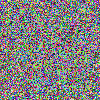
\includegraphics[width=0.5\columnwidth]{LMapStreamDinoDecrypted2.png}
		\caption{figure \ref{fig4} decrypted with r=3.996237151366785 }
		\label{fig7}
	\end{figure}


	\begin{figure}[htbp]
		\centering
		
\includegraphics[width=0.5\columnwidth]{HenonDinoDecrypted2.png}
		\caption{figure \ref{fig5} decrypted with  $x_0$=0.10415467387004729}
		\label{fig8}
	\end{figure}

	\begin{figure}[htbp]
		\centering
		\includegraphics[width=0.5\columnwidth]{SimpleDinoDecrypted2.png}
		\caption{figure \ref{fig5} decrypted with seed 444938}
		\label{fig9}
	\end{figure}


	Figures \ref{fig7}, \ref{fig8}, \ref{fig9} show attempts at decryption when modifiying certain initial conditions in the key.\\
	
	
	Finally, in Figures \ref{fig10} to \ref{fig14}, we report the image histograms of the encrypted images for each method in order to view the distribution of pixels in the image. The original image's histogram is also shown. The horizontal axis indicates the value of the specific color (in a range from 0 to 255), while the vertical axis indicates the frequency of that value.
	
	
	\begin{figure}[htbp]
		\centering
		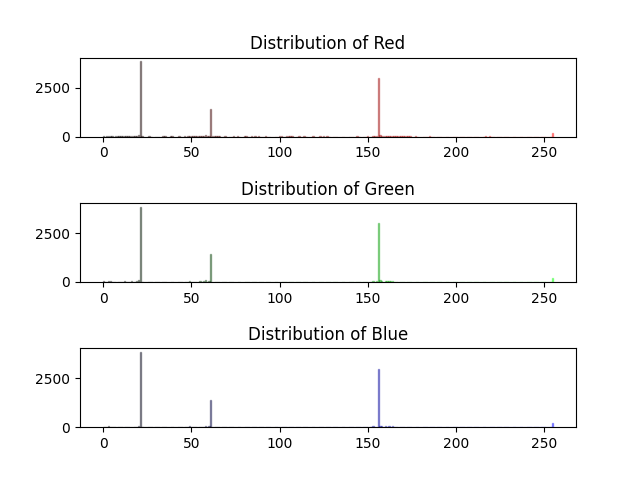
\includegraphics[width=0.95\columnwidth]{original_histogram.png}
		\caption{Distribution of colors of the original image to encrypt}
		\label{fig10}
	\end{figure}
	
	\begin{figure}[htbp]
		\centering
		\includegraphics[width=0.95\columnwidth]{SimpleDinoEncrypted_histogram.png}
		\caption{Distribution of colors when encrypted with simple XOR Cipher}
		\label{fig11}
	\end{figure}
	
	\begin{figure}[htbp]
		\centering
		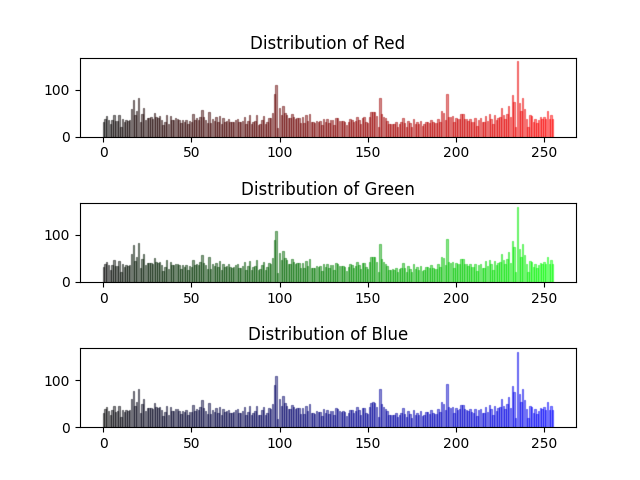
\includegraphics[width=0.95\columnwidth]{LMapStreamDinoEncrypted_histogram.png}
		\caption{Distribution of colors when encrypted with Logistic Map XOR Cipher}
		\label{fig12}
	\end{figure}
	
	
	\begin{figure}[htbp]
		\centering
		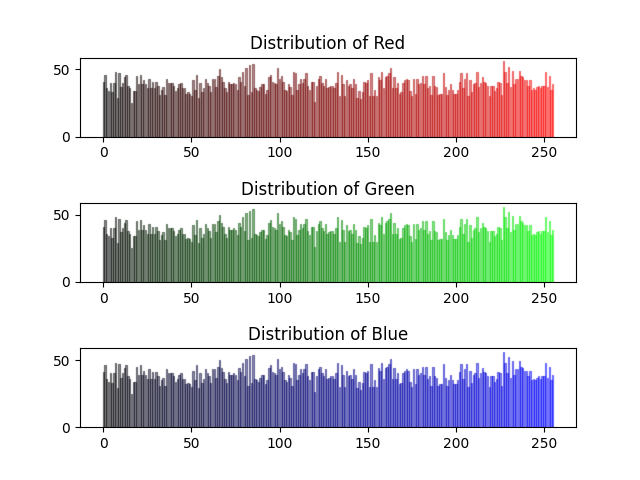
\includegraphics[width=0.95\columnwidth]{HenonDinoEncrypted_histogram.png}
		\caption{Distribution of colors when encrypted with Hénon Map Method}
		\label{fig13}
	\end{figure}
	
	
	\begin{figure}[htbp]
		\centering
		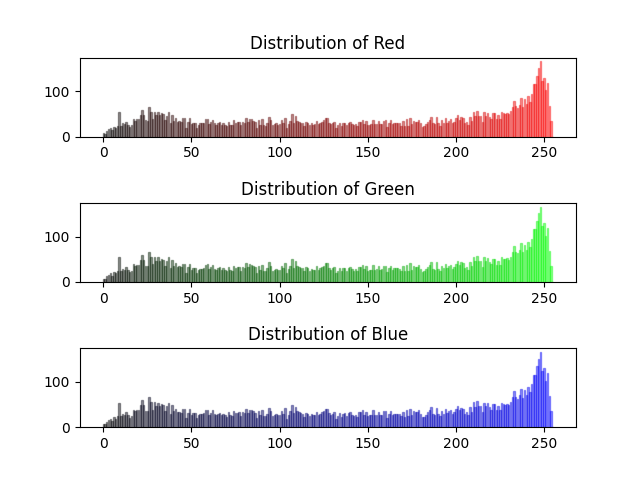
\includegraphics[width=0.95\columnwidth]{LMapPixelDinoEncrypted_histogram.png}
		\caption{Distribution of colors when encrypted with Logistic Map Pixel Iterations}
		\label{fig14}
	\end{figure}


	

    
    
    

    
    
    
    
    \section{Discussion}
    
    \subsection{Encryption and Decryption}
    Our results show that the simple methods we have outlined in this paper work relatively well to encrypt images. The original image is not distinguishable once encrypted. Nevertheless, when using the logistic map to generate a key for the stream cipher, a faint outline of the dinosaur remains as shown in Figure \ref{fig4}. Rounding numbers to integers between 0 and 255 may have affected the encryption results, as two different numbers generated by the logistic map could be converted to the same integer if they were close enough. These methods may have worked better on black-and-white images, where pixels have a value between 0 and 1. Finally, we note that Figure \ref{fig6} shows a slightly lighter complexion than the other encrypted images.
    
    \subsection{Image Histograms}
    
    In the image histograms, we would hope to see a uniform distribution of pixel values. More noise in the image would make it harder to spot patterns or other features to help decrypt it without the key. Figure \ref{fig11} and \ref{fig13} give us a good distribution of values. Unfortunately, when using the logistic map in Figure \ref{fig12}, there are clear spikes of frequency around certain values of red, green and blue. In Figure \ref{fig14}, we can also see evidence that the encrypted image is indeed lighter than the others. Many of its values are concentrated around 250. This shows that our methods are not perfect in terms of generating a completely ``random'' encrypted image.\\
    
    
    \subsection{Key sensitivity}
    
    In our Logistic Map Pixel Iteration method, we used different initial conditions for each pixel of the image, so it is clear that we do not have sensitive keys. A slight modification to one of the values of the original key results in an image that still resembles the original, since every pixel is calculated independently of the others.
    
    However, the results show very good key sensitivity for the rest of our methods. Chaotic maps are sensitive to initial conditions, so this is not totally unexpected. This means that an attacker would not know ``how close'' they are to the true key when attempting, say, a brute-force attack.
    
    \subsection{Runtime performance}
    
    All methods tested in this paper ran extremely quick ($< 0.1s$) except for the method in \ref{ssec:n2}. This approach's runtime heavily depends on the parameter $N$. With small values at $N \in [5, 15]$, it took about 20 seconds for a single 100x100 image. With larger $N$ in the range of 100 to 200, it took up to 5 or 6 minutes. This makes it nearly unusable in real-time applications.\\
    
    The logistic map pixel iteration method occupies a very large keyspace, as the key itself is the set of parameters for \textit{each pixel} of the image. If we let $R, |N|, |C|, |L|$ be the number of possible values for the parameters $r, N, C$ and $L$ respectively, we would have $3R|N||C||L|mn$ possible values for the key.
    
    In contrast, the cryptographic keyspace for the XOR methods do not scale proportionally to the size of the image as the key is based on initial conditions. For example, for the logistic map XOR method, we only save $r$, $x_0$ and an integer offset. The keyspace is then constrained by the number of values the floats can take (language dependent) and the number of values the integer can take (usually $2^{31} -1$). 
    
    
    
    \subsection{Conclusion}
    
    Overall, image encryption can be a complicated topic with many considerations at play. Using a discrete chaotic map to generate a sequence of integers for an XOR Cipher may not always work in all aspects, as we have seen. When considering the use of chaotic maps in image encryption, one cannot simply plug them into basic/simplified methods of encryption and expect them to work perfectly. In the future, more work would be needed to elaborate better schemes that involve discrete chaotic maps.
    
    Furthermore, the new method we have proposed in this paper does not seem very useful in real-time applications. It would be too slow without much benefit elsewhere. As it is not key sensitive and its distribution of encrypted colors seems skewed, further work is needed before we could actually use this.
    
    \section{References}
    \begingroup
    \renewcommand{\section}[2]{}%
    %\renewcommand{\chapter}[2]{}% for other classes
    \bibliographystyle{ieeetr} 
    \bibliography{references}
    \endgroup
    
    \renewcommand{\thesection}{\Alph{section}}
    \setcounter{section}{0}
    
    \section{Appendices} \label{sec:app}
    
    To verify our results, we tested our methods on a second image. In this section, we show examples of encryption results on an image of a 100x100 penguin. To view the full results, readers may consult section \ref{sec:supp}.
    
    \begin{figure}[htbp]
    	\centering
    	
\includegraphics[width=0.5\columnwidth]{penguin.png}
    	\caption{A second example of an 100x100 image to encrypt}
    	\label{fig15}
    \end{figure}
    
    
    
     \begin{figure}[htbp]
    	\centering
    	
\includegraphics[width=0.5\columnwidth]{simplePenguinEncrypted.png}
    	\caption{Penguin encrypted with simple XOR Cipher}
    	\label{fig16}
    \end{figure}
    
    
    \begin{figure}[htbp]
    	\centering
    	
\includegraphics[width=0.5\columnwidth]{simplePenguinDecrypted.png}
    	\caption{figure \ref{fig16} decrypted with simple XOR Cipher}
    	\label{fig17}
    \end{figure}
    
    
    
    \begin{figure}[htbp]
    	\centering
    	
\includegraphics[width=0.5\columnwidth]{LMapStreamPenguinEncrypted.png}
    	\caption{Penguin encrypted with Logistic Map XOR Cipher}
    	\label{fig18}
    \end{figure}
    
    
    \begin{figure}[htbp]
    	\centering
    	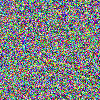
\includegraphics[width=0.5\columnwidth]{HenonPenguinEncrypted.png}
    	\caption{Penguin encrypted with Hénon Map Method}
    	\label{fig19}
    \end{figure}
    
    
    \begin{figure}[htbp]
    	\centering
    	
\includegraphics[width=0.5\columnwidth]{LMapPixelPenguinEncrypted.png}
    	\caption{Penguin encrypted with Logistic Map Pixel Iterations}
    	\label{fig20}
    \end{figure}
    

    
    
    \section{Supplementary Material} \label{sec:supp}
    
    A demonstration of certain encryption experiments carried out in this paper can be found at the following website: \href{https://logistic-map-326.herokuapp.com/}{https://logistic-map-326.herokuapp.com/}.\\
    
    The website allows users to input a PNG image and encrypt it using any of the methods described in this paper. Users can also decrypt an image by indicating the correct key. The parameters are preset for all models of encryption to some default values.\\
    
    The source code to reproduce the results is also available at the following repository: \href{https://github.com/WiIIiamTang/logistic-map-encryption/tree/main/chaosencryptor}{https://github.com/WiIIiamTang/logistic-map-encryption/tree/main/chaosencryptor}. The full results and additional images can be found here.
 
\end{document}